\documentclass{standalone}
\usepackage{tikz}


\begin{document}
% set up the main coordinate frame
\pgfmathsetmacro{\thetaXt}{50}
\pgfmathsetmacro{\phiZ}{135}
\tdplotsetmaincoords{\thetaXt}{\phiZ}

% rotate reference frames according to the Z, Y, X order instead of the default Z, Y, Z
\tdseteulerxyz

\begin{tikzpicture}[tdplot_main_coords] 
\pgfmathsetmacro{\axissize}{5}
\pgfmathsetmacro{\linewidth}{3}
\linespread{1}
\coordinate (O) at (0,0,0);
\node at (O){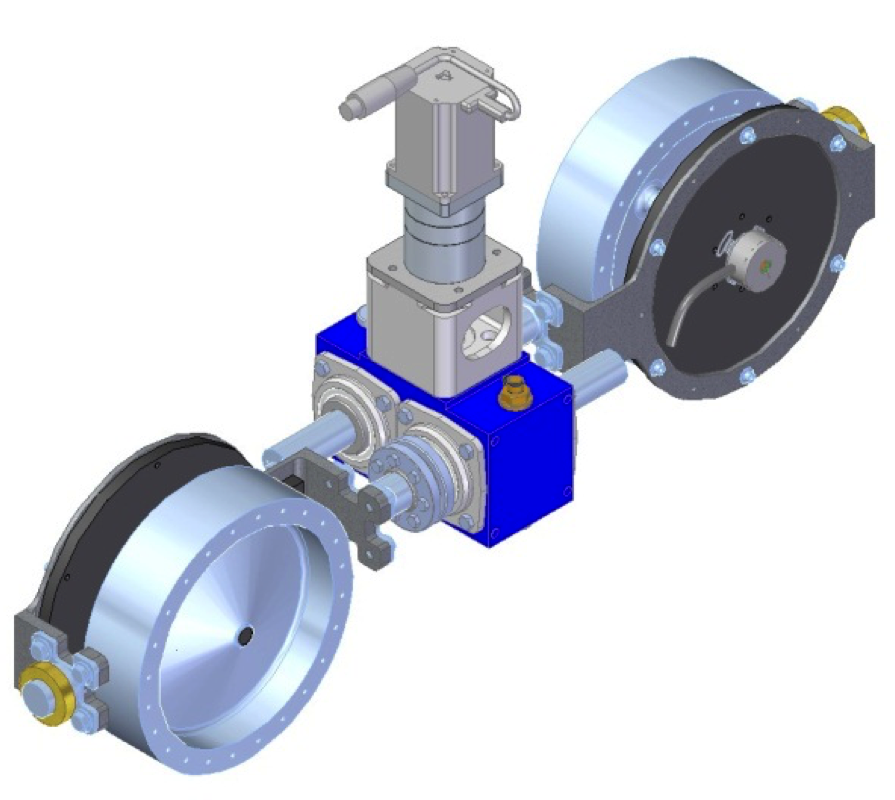
\includegraphics[width=\textwidth]{Figures/CCMG-nocase.png}};

\draw[->,red,line width=\linewidth] (O) -- (0,0,\axissize)node[right]{\vectors{z}};
\draw[->,red,line width=\linewidth] (O) -- (0,\axissize,0)node[right]{\vectors{x}};
\draw[->,red,line width=\linewidth] (O) -- (-\axissize,0,0)node[below]{\vectors{y}};

\coordinate (V) at (6.75,2,0);
\draw[->,red,line width=\linewidth] (V) -- (6.75,7,0)node[below]{}node[midway]{\AxisRotator[rotate=-30,->]};
\coordinate (V2) at (-6,-1,0);

\draw[->,red,line width=\linewidth] (V2) -- (-6,-8,0)node[below]{}node[pos=0.4]{\AxisRotator[rotate=-30,<-]};


\node[above] at (6,-3,1){Wheel A};
\node[below] at (-6,3,-1){Wheel B};
\node[left] at (1,-1,5.5){Stepper motor};
\node[left] at (1,-1,3){Gear box};

\draw[->,red,line width=\linewidth] (9,0.7,0) -- (12,0.7,0)node[pos=0.7]{\AxisRotator[rotate=30,->,dashed]}node[pos=0.8,below=2em,align=center]{Gimbal \\ rotation};

\end{tikzpicture}
\end{document} 